\chapter {Cloud Approach}
In this chapter we introduce the collective entity matching problem and give our solution to implement it on the cloud. We start by giving a a simple example, theoretical foundation, and then we explain the different components of our solution.

\section{Simple Example}
As an example we use a bibliographical example presented by Bhattacharya and Getoor\cite{BhGe06b}. In this example we consider the problem of resolving the authors in academic publications databases like DBLP and CiteSeer. Consider the following set of four papers:

\begin{enumerate}
\item A. V. Aho, S. C. Johnson, J. D. Ullman, "code generation for machines with multi-register operations"
\item A. V. Aho, J. D. Ullman, "The university of database languages"
\item A. V. Aho, J. D. Ullman, "Optical partial-match retrieval when fields are independently specified"
\item Alfredo V. Aho, Jeffrey D. Ullman, Scott Johnson, "Code generation for expressions with common sub-expressions"
\end{enumerate}

We would like to find out, given these papers, which of the referenced author names belong to the same author entities. For instance we need to determine whether paper 1 and paper 2 are written by the same author named Ullman, or whether the name references belong to different authors. The same need to be considered for the Ullman from paper 3 and Ullman from paper 4, and all pairwise combinations. Similar questions about the author names Johnson and Aho also need to be considered in this context. 

In order to resolve these authors references, we may begin by examining the author references to see which ones we consider to be the same. In the first step we might decide that all of the Aho references refer to the same author entity because Aho is an unusual last name. This corresponds to resolving all the Aho references into a single entity. However, we might be not quite sure that the Ullman references are the same author, and we certainly not sure about Johnson references, since Johnson is very common name. But deciding that the Aho references correspond to the same entity gives us additional information for the Ullman references. We know that the references share a common co-author. Now with a higher confidence we can consolidate the Ullman references. Based solely on the Aho entity consolidation, we do not have enough evidence to consolidate the Johnson references. However, after making the Ullman consolidations, we may decide that having two co-authors in common is enough evidence to tip the balance, and that all the Johnson references correspond to the same Johnson entity Figure \ref{fig:shaded_ref}.b. We end up having three author entities. We will call these entities \textit{Alfred V Aho}, \textit{Jeffrey D Ullman}, and \textit{Scott Johnson}. This is illustrated by figure ~\ref{fig:shaded_ref}(b), where references correspond to the same authors are shaded identically.

\begin{figure}
\centering
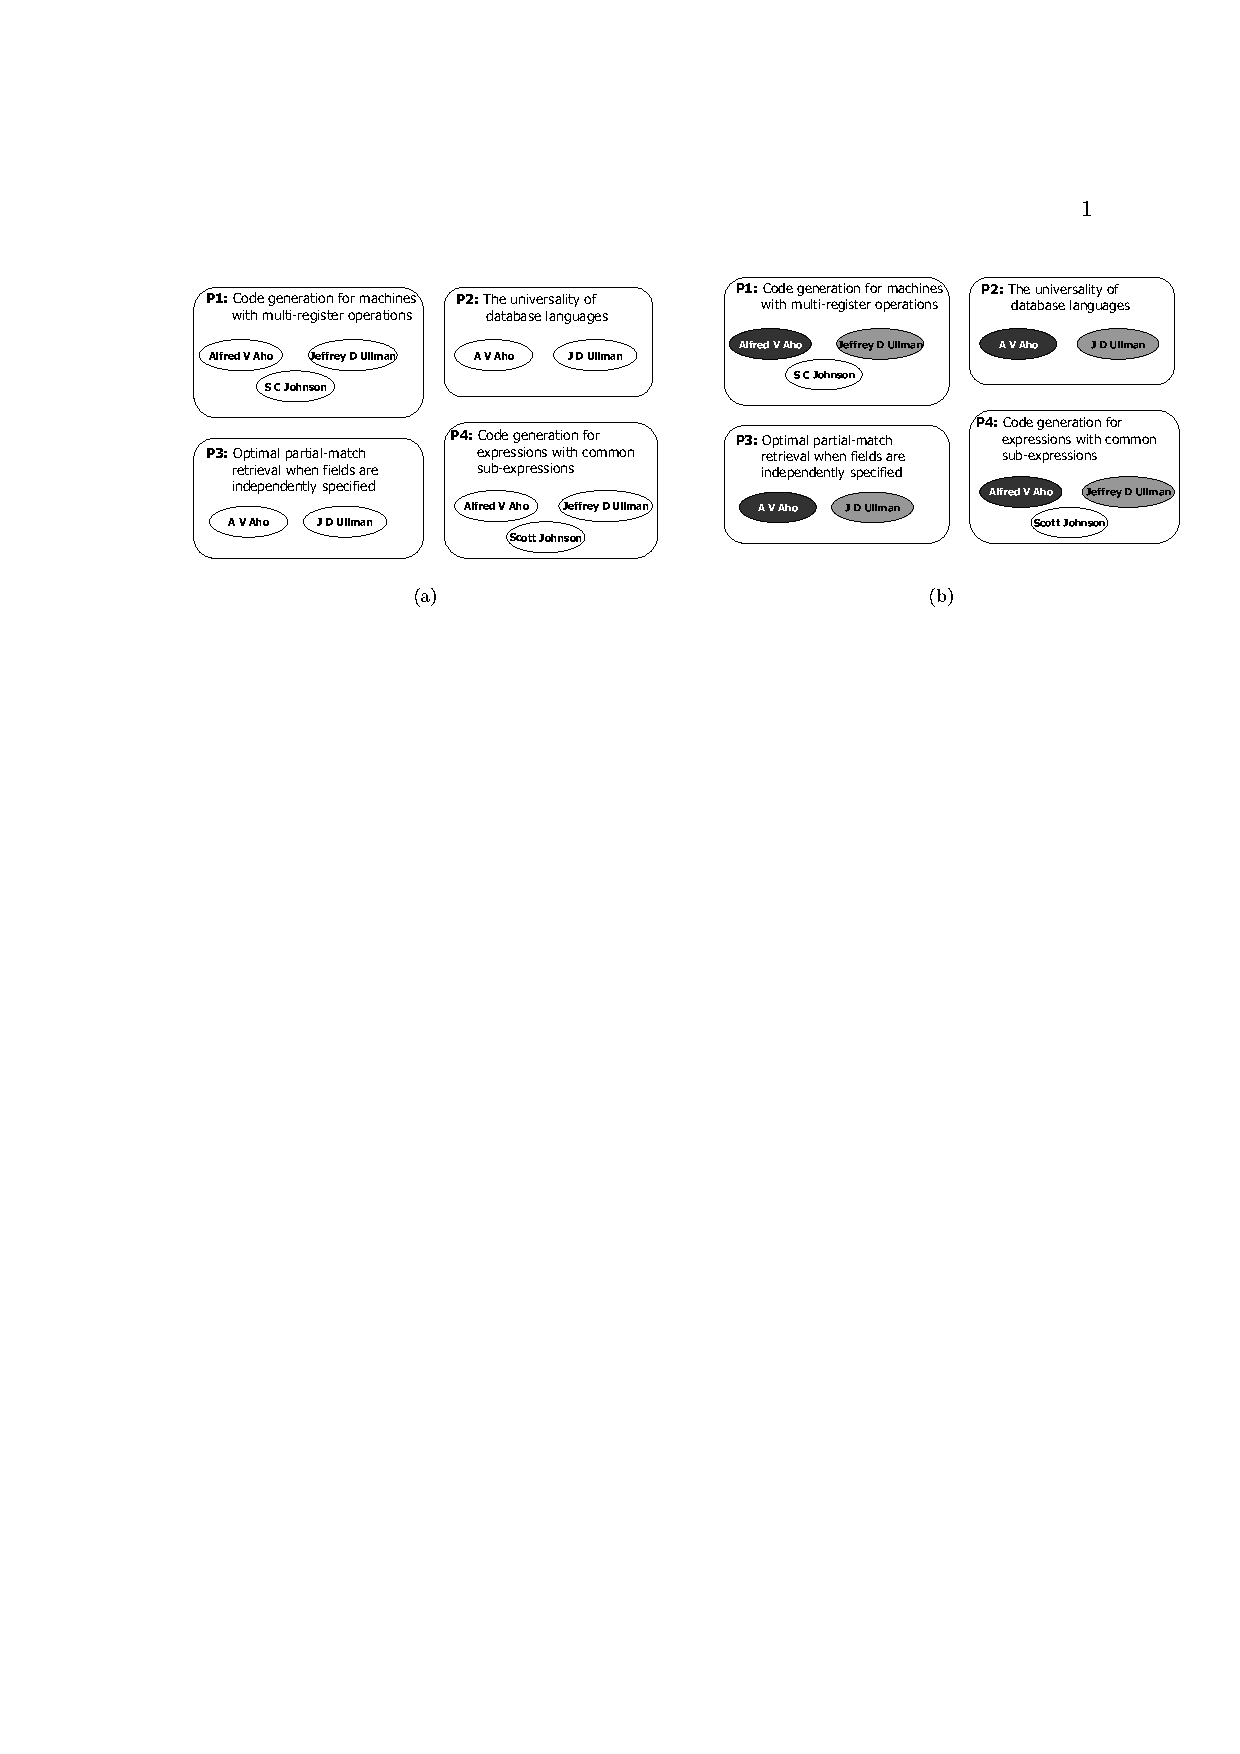
\includegraphics[page=1,trim = 32mm 190mm 0mm 45mm, clip]{figures/chapter3/fig1_ab_cliping}  
\caption{(a) An example author/paper resolution problem. Each box represents a paper reference and each oval represents an author reference. (b) The resolved entities corresponding to the example author/paper resolution problem. (\cite{BhGe06b})}
\label{fig:shaded_ref}
\end{figure}  

In this example we can find instances of an identification problem. The identification problem can be seen in the references with different names which refer to the same entity. For example entity author 'Jeffery David Ullman' might be referenced as 'J. D. Ullman', 'Jeffery D. Ullman', 'J. Ullman' and so on. another problem we might find is the disambiguation problem which can be seen in references that have the exact same names but refer to different entities.

To solve the identification and disambiguation problems, relationships between references can be used to better resolve the references to their corresponding real entities \cite{BhGe07}. These relationships can be represented as a graph where nodes represent the references and the hyper-edges represent the relationships between references. In our example the graph can be constructed such that  the nodes represent the authors and the hyper-edges represent the co-authorship relation that hold between them. Figure ~\ref{fig:ref_ent}(a) shows the reference graph for our bibliographic example. Given this graph representation for our data, our goal is to take into consideration the hyper-edges to better partition the references into entities. This can gives better results because references with similar or exact names are more likely to be the same entity if their hyper-edges connect to the same entities as well. We can see this in our example (figure ~\ref{fig:shaded_ref}), first observe that the Ullman references collaborate with Aho's who correspond to the same author. This make it more likely that they are the same entity. From the relationship graph between the references we incrementally constructs the entity graph by considering as evidence the entity relationships that it has already discovered earlier. Figure ~\ref{fig:ref_ent}(b) shows the resulting entity graph for our example after all the references have been correctly resolved.

\begin{figure}%[ht!]
\centering
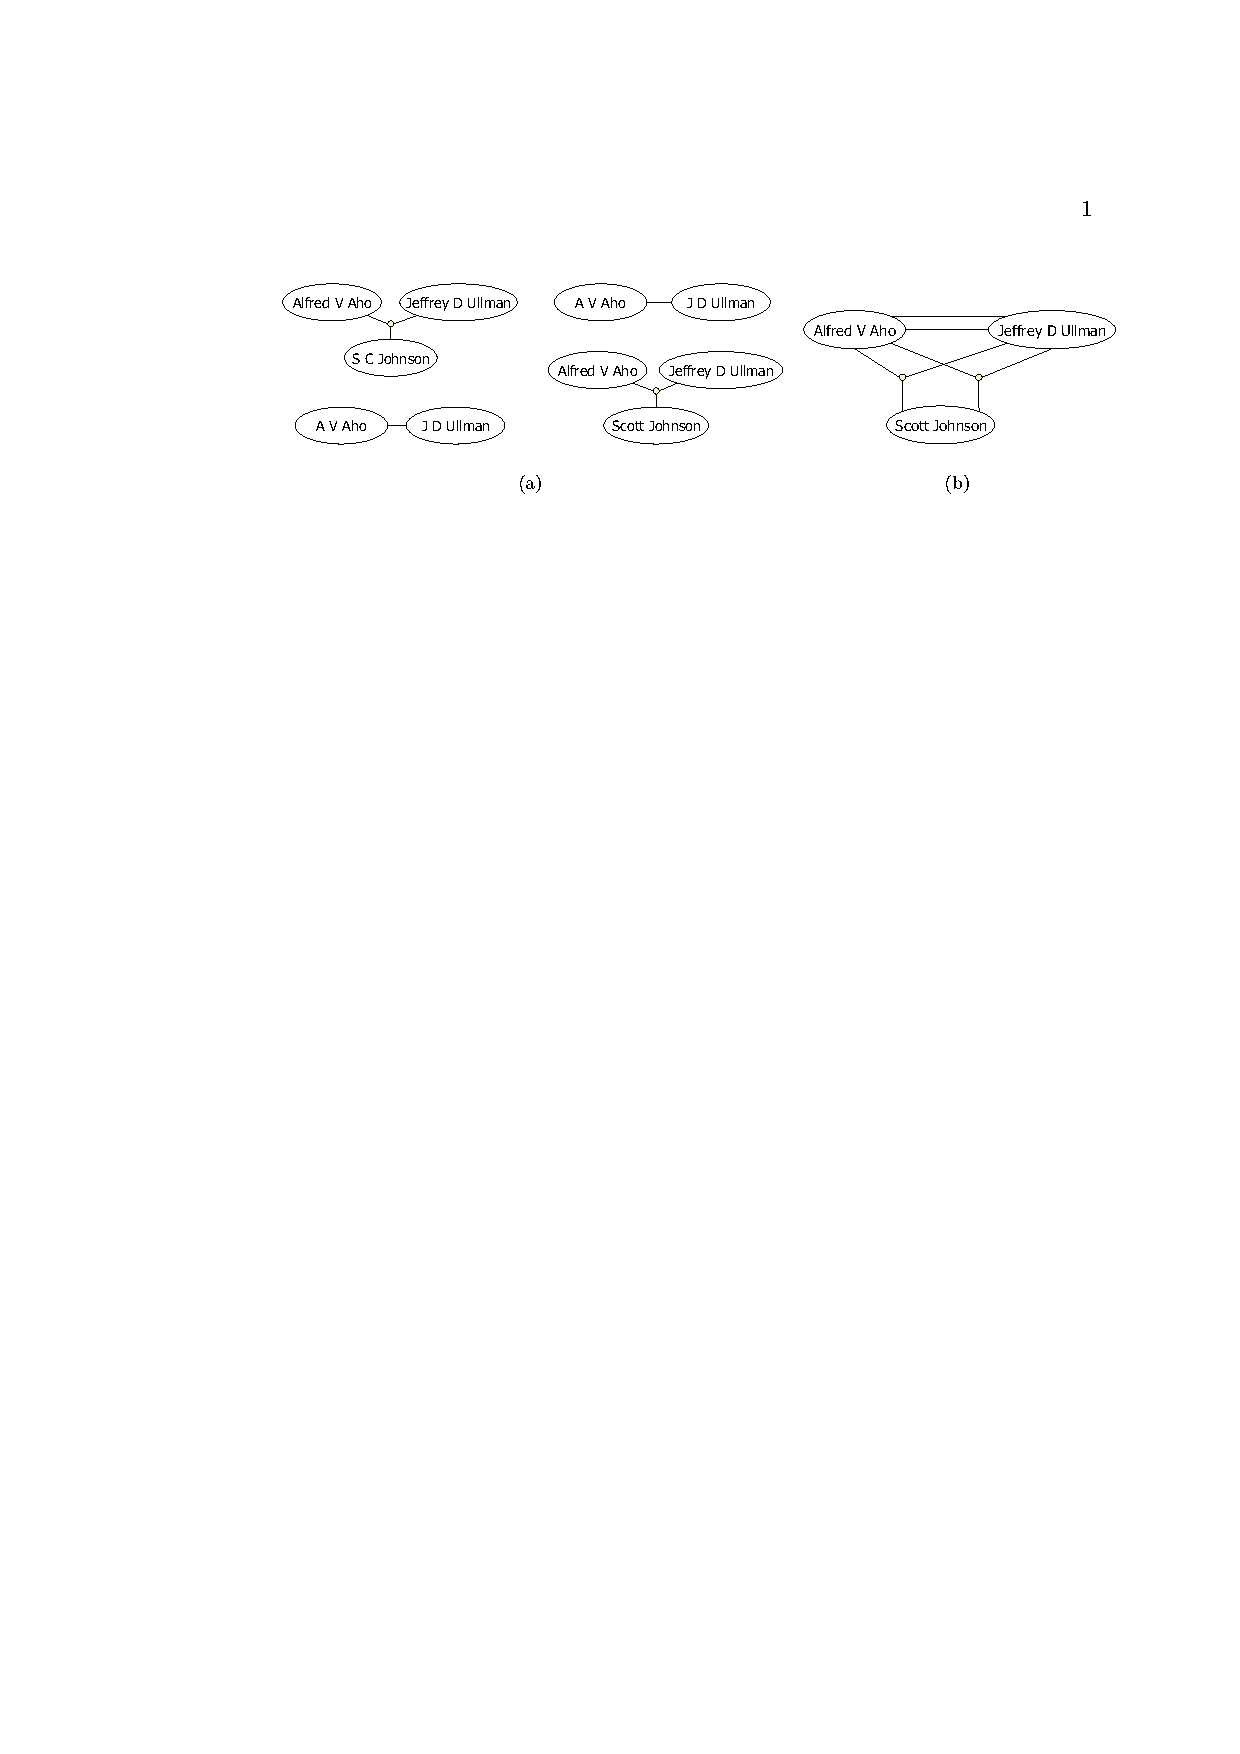
\includegraphics[page=1,trim = 35mm 210mm 0mm 45mm, clip]{figures/chapter3/fig2_ab_cliping}
\caption{(a) The reference graph and (b) the entity graph for the author resolution example. (\cite{BhGe07})}
\label{fig:ref_ent}
\end{figure}  

\section{Theoretical Foundation}

In this section, we introduce the notation to be used for describing the relational entity matching problem based on the work of Bhattacharya and Getoor\cite{BhGe07}.
 
To formalize the problem we need notations for references, entities and hyper-edges. In the entity resolution problem, we are given a set of references $\mathcal{R}=\{r_i\}$, where each reference $r$ has attributes $r.A_1,r.A_2,...,r.A_k$. The references correspond to some set of unknown entities $\mathcal{E} = \{e_i\}$. We introduce the notation $r.E$ to refer to the entity to which reference $r$ corresponds.

 The problem is to recover the hidden set of entities $\mathcal{E} = \{e_i\}$ and the entity labels $r.E$ for individual references given the observed attributes of the references.In the context of collective entity matching, we assume that the references are not observed independently, but that they co-occur. We describe the co-occurrence with a set of hyper-edges $\mathcal{H} =\{h_i\}$. Each hyper-edge h may have attributes as well, which we denote $h.A_1,h.A_2,...,h.A_l$, and we use $h.R$ to denote the set of references that it connects. A reference $r$ can belong to zero or more hyper-edges and we use $r.H$ to denote the set of hyper-edges in which $r$ participates. Considering again out example, we can see how this notation is represented.

Lets show how this applies to our example, Figure \ref{fig:abs_ent}(a) shows the references and hyper-edges. Since each author name corresponds to a reference, then there are ten references $r_1$ through $r_{10}$. In this case, the the attributes are the names themselves, so for example $r_1.A$ is "Alfred Aho", $r_2.A$ is "S. C. Johnson" and $r_3.A$ is "Jeffrey Ullman". Now considering the entities, we have a set of true entities as shown in figure \ref{fig:abs_ent}(b). where $e_1.A=$"Alfred V. Aho", $e_2.A=$"S. C. Johnson" and $e_3.A=$"Jeffrey D. Ullman". We observe that references $r_1$, $r_4$, $r_6$ and $r_8$ correspond to "Alfred V. Aho", so that $r_1.E = r_4.E = r_6.E = r_8.E = e_1$. In similar way, we observe that $r.3:E = r_5.E = r_7.E = r_10 = e_2$ and $r_2.E = r_9.E = e_3$. 
Now considering the Hyper-edges, we have hyper-edges $\mathcal{H} = \{h_1,h_2,h_3,h_4\}$, one for each paper. The attributes of  the hyper-edges in this domain are the paper titles; for example, $h_1.A_1=$"Code generation for machines with multi-register operations". The references $r_1$ through $r_3$ are associated with hyper-edge $h_1$, since they are the observed author references in the first paper. This is represented as $h_1.R = \{r_1,r_2,r_3\}$. We similarly represent the hyper-edge associations of the other references. The problem here is to figure out from the attributes $r.A$ and the hyper-edge label $r.h$ of the references that there are three distinct entities such that $r_1,r_4,4_6$ and $r_8$ corresponds to one entity, $r_3,r_5,r_7$ and $r_10$ correspond to the second entity and $r_2$ and $r_9$ correspond to the third. Here we have introduced the notation assuming that all references correspond to the same class of entities, It may be extended to handle multiple entity classes and multiple types of hyper-edges between references.

\begin{figure}%[ht!]
\centering
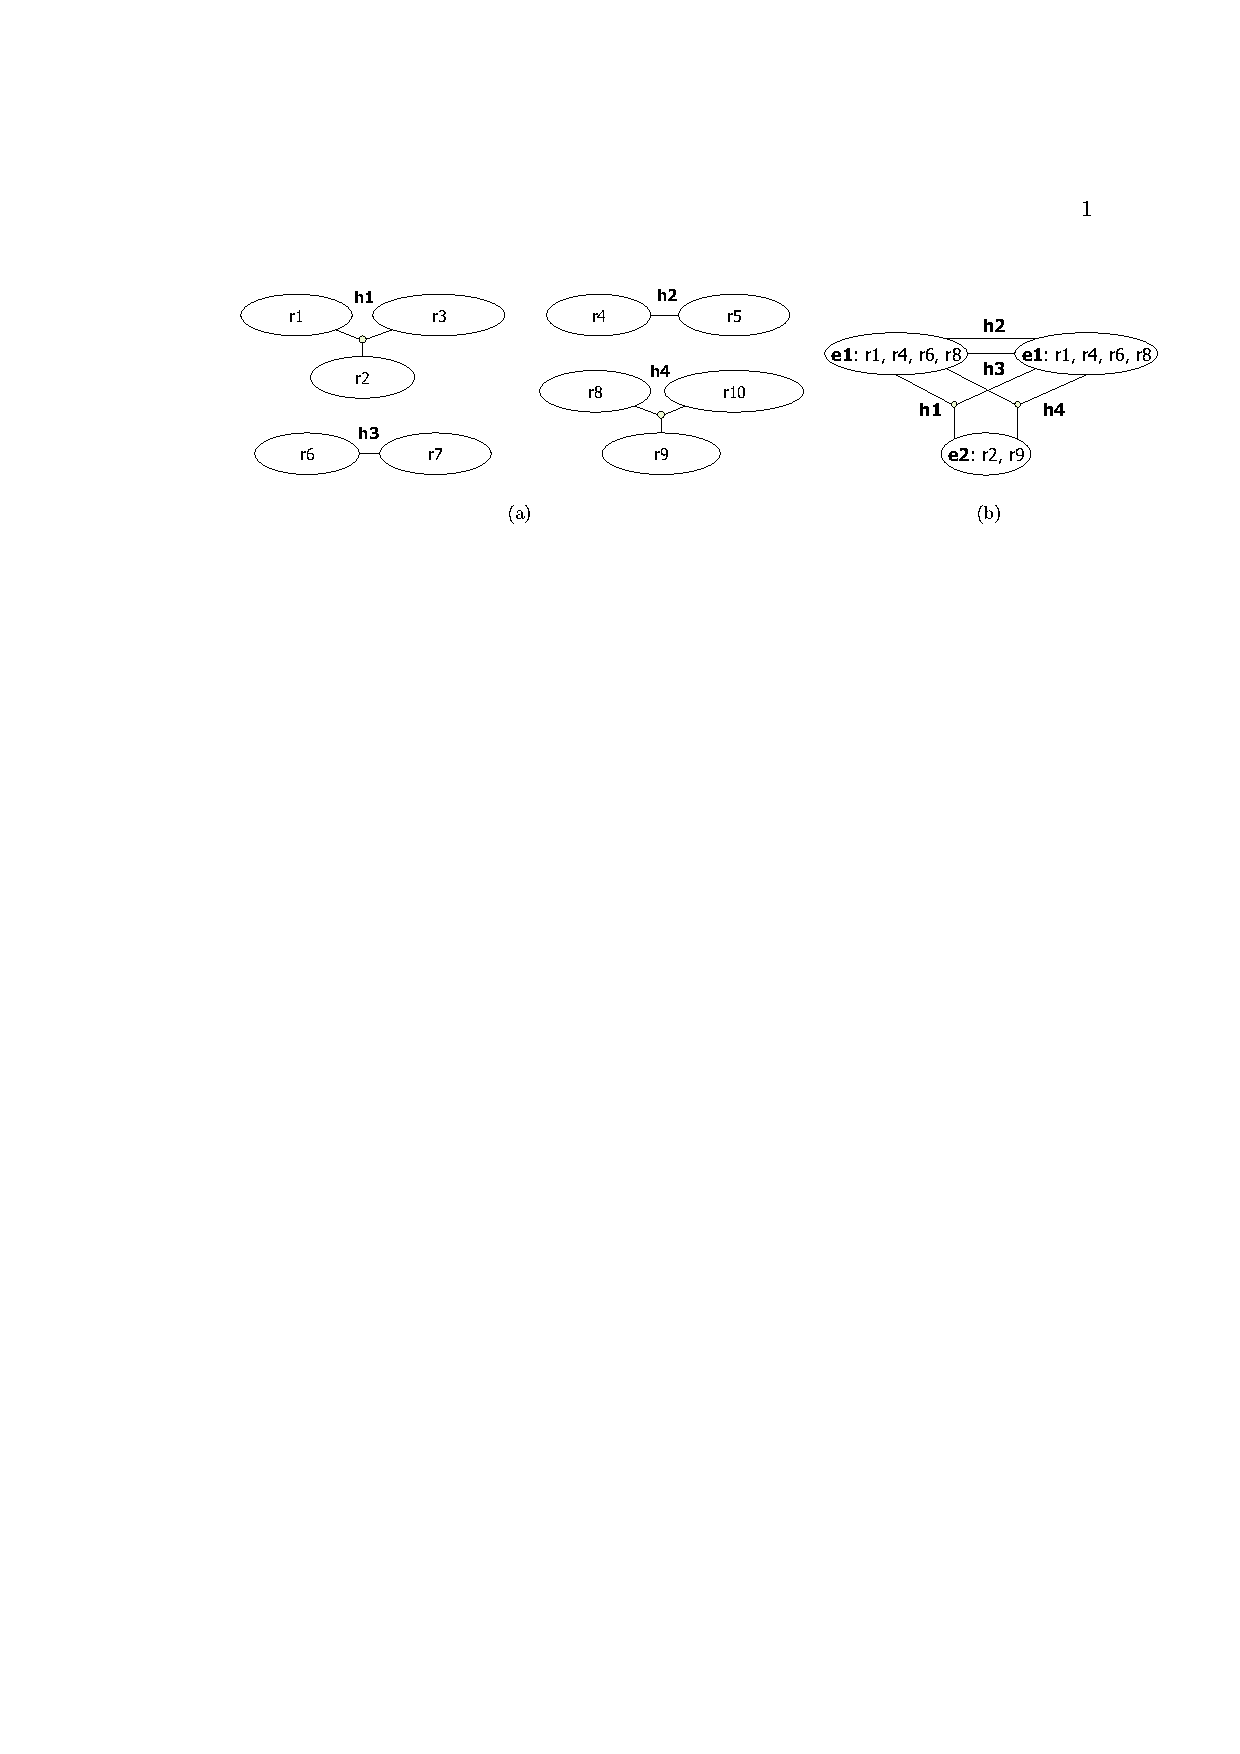
\includegraphics[page=1,trim = 35mm 205mm 0mm 45mm, clip]{figures/chapter3/fig3_ab_cliping} 
\caption{(a) A more abstract representation of the reference graph for the author resolution example; the r's are references and the h's are hyper-edges. (b) An abstract representation for the entity graph for the author resolution example; the nodes are the entities, the set of references they correspond to are listed, and the h's are hyper-edges.. (\cite{BhGe07})}
\label{fig:abs_ent}
\end{figure}  
\section{Proposed Solution}
In this section we describe the solution approach . The solution approach consists of several stages as shown in figure \ref{fig:SolutionAppraoch}. We give an overview of each stage and discuss the problems need to be solved in each stage.

\begin{figure} [H]
\centering
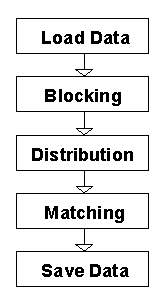
\includegraphics{figures/chapter3/fig0_ApproachBlockDiagram.eps}  
\caption{Block Diagram of the Solution Approach}
\label{fig:SolutionAppraoch}
\end{figure}

\subsection{Load Data}
In load data stage. Data from different sources having different formats need to be loaded into the framework.
\subsection{Blocking}
In this stage, the loaded data need to be blocked such that similar entities are grouped into blocks. The blocks may overlap with each other. Figure \ref{fig:bloking_example} shows the references to authors grouped into blocks.

\begin{figure}[H]
\centering
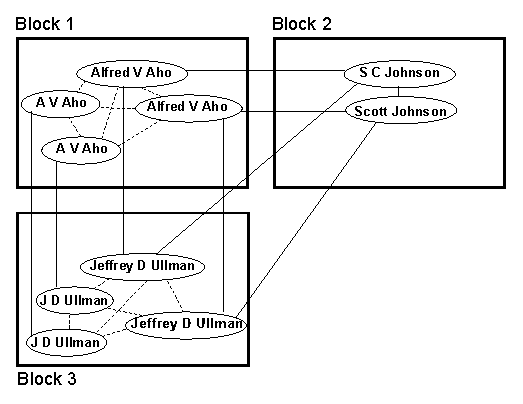
\includegraphics{figures/chapter3/fig_blocking_example.eps}  
\caption{Blocking of the reference graph (solid: links to neighbor references, dashed: links to references in the same block) }
\label{fig:bloking_example}
\end{figure}

\subsection{Distribution}
After the data records are grouped to overlapped blocks (canopies), we need to distribute the data over the machines of the cloud. the distribution should be balanced and should also ensure that overlapped blocks reside in the same machine. To illustrate that we added more author references to our running example. The new author references are grouped in \textit{block4} and \textit{block5}. \textit{block5} overlaps with both \textit{block2} and \textit{block4}. The blocks are distributed among two machines such that overlapped blocks resides in single machine and the blocks distribution among the two machines is balanced as much as possible (see figure \ref{fig:distributedBlocks_example}).

\begin{figure}[H]
\centering
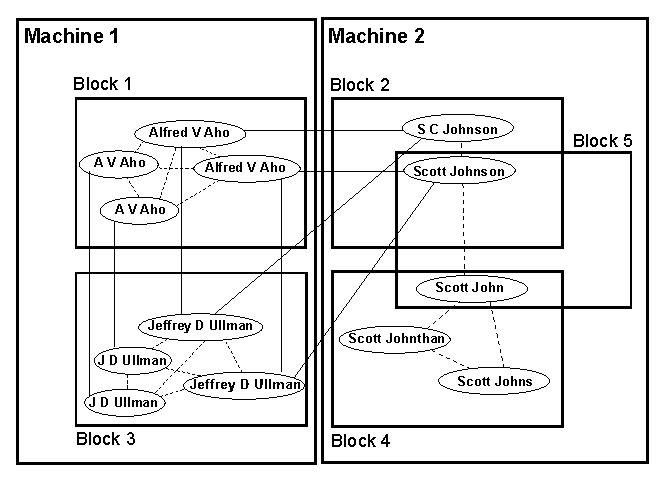
\includegraphics{figures/chapter3/fig_overlapedBlocks_machines.eps}  
\caption{Overlapped blocks should reside in single machine}
\label{fig:distributedBlocks_example}
\end{figure}


\subsection{Matching}
In this stage, the blocked data records that have similarity measure above the user defined threshold will be merged. We use the Collective relational entity matching approach and implement it on Pregel.
\subsection{Save Data}
After the data is matched, we need to store the results. statistical and log files should also be stored.

\section{Blocking}
For data blocking, we implement the meta-blocking general procedure proposed by Papadakis et al. \cite{GGT*13} to create and process the blocks. In meta-blocking, The initial set of blocks is transformed into a new one with substantially fewer comparisons and equally high effectiveness. The new set of blocks is constructed from the most similar pairs of entities. The procedure starts by building an abstract graph representation of the original set of blocks. In this graph, the nodes correspond to entity references and the edges connect the co-occurring ones. During the creation of this structure all redundant comparisons are discarded, while the superfluous ones can be removed by pruning of the edges with the lowest weight.
This blocking procedure is built upon an idea from redundancy-positive blocking techniques. In redundancy-positive blocking techniques, the number of common blocks between a pair of entity profiles is proportional to their similarity and, thus, the likelihood that they are matching. So the more blocks two entity references share, the more likely they are to describe the same real-world entity. Its interesting to notice that this is a contrary to the redundancy-negative Canopy clustering technique used in the original Collective entity matching approach\cite{GGT*13}.

The efficiency of redundancy-positive blocking methods can be improved by discarding the unnecessary comparisons of their blocks. In general, comparisons of this kind are distinguished into two categories: (i) the redundant ones, which repeatedly compare the same entities across different blocks, and (ii) the superfluous ones, which involve non-matching entities\cite{GGT*13}. 

We can mainly enhance the efficiency of redundancy-positive blocking methods by operating at the coarse level of entire blocks. We use Block Purging \cite{PIN*11} to a-priori discards \textit{oversized blocks}, which involve an excessively high number of unnecessary comparisons.
A similar technique is Block Pruning \cite{PIN*11}. This technique assumes an ordered set of blocks and terminates their processing as soon as duplicate overhead (i.e., the cost of identifying new duplicates) exceeds a predefined threshold\cite{GGT*13}.

Meta-blocking operates efficiently because it skips the high complexity of computing pair-wise, string-based entity similarities, relying instead on the block-to-entity profile associations of the input set of blocks\cite{GGT*13}.
\section{Distribution}
\begin{comment}
Assume that we have 2 machines and 5 block $b_1,b_2,...,b_5$. $b_1$ overlaps with $b_2$ and $b_3$. The blocks elements are as follows:\\ 
$b_1=\{a,b,c,d\}$\\
$b_2=\{a,b,e\}$\\ 
$b_3=\{c,f,g\}$\\
$b_4=\{o,p,q,r,s\}$\\  
$b_5=\{w,y,z\}$\\

Since the blocks $b_1$,$b_2$ and $b_3$ overlaps, they should reside in one machine. The other blocks that do not overlap with each other can reside in any other machine. since we aim to have balanced distribution, they reside in the second machine. figure \ref{fig:fig_distribution_example} shows the required distribution of the blocks.
\begin{figure}[H]
\centering
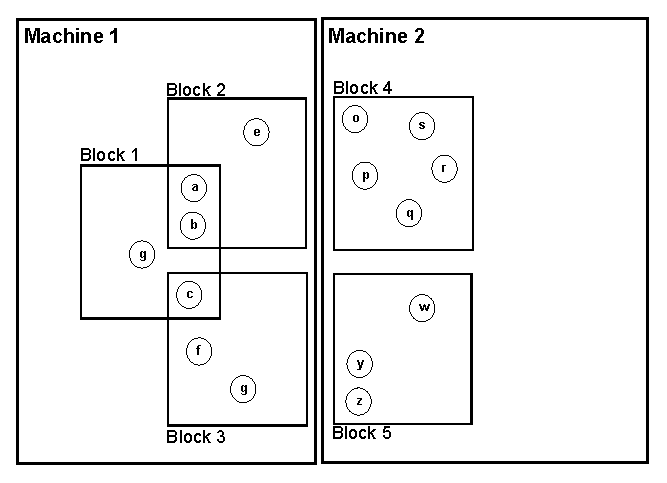
\includegraphics{figures/chapter3/fig_distribution_example.eps}  
\caption{overlapped blocks should reside in single machine}
\label{fig:fig_distribution_example}
\end{figure}
\end{comment}
Good partitioning of input data is a key prerequisite for parallel entity matching since it influences processor utilization, communication overhead, and load balancing\cite{KKH*10}. Since our algorithm is communication intensive, having good data partitioning is critical to have a local communication overhead centered in the machines of the cloud such that networking overhead is minimized.

To partition the input data we use a block-based partitioning approach proposed by Kirsten et. al. \cite{KKH*10}. This approach is called \textit{partition tuning} and it split or combine blocks as following:
\begin{itemize}
\item We start by determining all large blocks for which the memory requirements exceed the maximum allowed size. We split these block into several equally sized partitions that obey the size restriction.
\item Then we aggregate all smaller blocks that have size below some fraction of the maximal partition size into larger ones.
\end{itemize}



\section{Matching by Collective Relational Entity Matching}
Our solution approach is based on the collective relational entity matching introduced by Bhattacharya and Getoor\cite{BhGe07}. The main key idea of collective relational entity resolution,  is that resolutions are not made independently, but instead one resolution decision affects other resolutions via hyper-edges\cite{BhGe06b}.
 
In this approach, a relationship graph is built where references are represented as nodes and relationships between these references are represented as edges between corresponding nodes. The edges can be between more than two nodes (called hyper-edges). The similarity between two nodes is calculated as the weighted sum between attribute value similarity and the relational similarity. The relational similarity is calculated based on the connectivity of the two nodes through their hyper-edges as well as the connectivity of the neighboring nodes they are connected to. For collective entity resolution, we define the similarity of two clusters $c_i$ and $c_j$ as\cite{BhGe06b}:

%\begin{align*}
$$sim(c_i,c_j)=(1-\alpha) \times sim_A(c_i,c_j) + \alpha \times sim_R(c_i,c_j), 0\leq\alpha\leq1$$
%\end{align*}

where $sim_A()$ is the similarity of attributes and $sim_R()$ is the relational similarity between references in the two entity clusters. The relational similarity $sim_R()$ is dynamic in nature, which is one of the most important and interesting aspects of the collective approach\cite{BhGe07}. Worth to notice here that for collective resolution, the similarity of two clusters depends on the current cluster labels of their neighbors, and therefore changes as their labels are updated.

For collective entity resolution, relational similarity considers the cluster labels of all these connected references. Recall that each reference $r$ is associated with one or more hyper-edges in $\mathcal{H}$. Therefore, the set of hyper-edges $c.H$ that we need to consider for an entity cluster c is defined as\cite{BhGe07}:
%\begin{align*}
$$c.H= \bigcup_{r\in R \wedge r.C=c}\{h|h\in \mathcal{H} \wedge r \in h.R\}$$
%\end{align*} 
Cluster $c$ is connected to other clusters by these hyper-edges. For any cluster $c$, the set of other clusters to which $c$ is connected via its hyper-edge set $c.H$ form the neighborhood $Nbr(c)$ of cluster $c$\cite{BhGe07}:
%\begin{align*}
$$Nbr(c)= \bigcup_{h\in c.H,r\in h.R}\{c_j|c_j=r.C\}$$
%\end{align*} 

\begin{comment}
%This defines the neighborhood as a set of related clusters.
\subsection{Attribute Similarity Measures}
As we see, we need to measure the similarity of the attributes. A wide variety of measures exists. They can be categorized to character-based similarity measures, token-based similarity measures, phonetic similarity measures and numeric similarity measures \cite{EIV07}. We use SimMetrics, which is a Similarity Metric Library, that provide several measures from edit distance's (Levenshtein, Gotoh, Jaro etc) to other metrics, (e.g Soundex, Chapman). 
Specific Attribute similarity measures that is important to us are the following:

\subsubsection{Soft TF-IDF}
Soft TF-IDF similarity can be used for names since it has been shown to perform well for name-based entity resolution. Essentially, Soft TF-IDF augments the TF-IDF similarity for matching token sets with approximate token matching using a secondary string similarity measure \cite{BhGe07}.

\subsubsection{Jaro-Winkler}
Jaro-Winkler is reported to be the best secondary similarity measure for Soft TF-IDF. It is well-suited for short strings such as personal names \cite{BhGe07}

\subsubsection{Scaled Levenstein}
Scaled Levenstein belongs to the edit-distance family of similarity measures that assigns unit cost to each edit operation and normalizes the result \cite{BhGe07}.

\subsubsection{Cosine similarity}

\subsection{Neighborhood Similarity Measures} 
As we have seen, the relational similarity between two clusters can be calculated by the considering the similarity of their neighborhoods. Many different metrics have been proposed and evaluated in literature. In this section introduce some these measures and study their applicability for entity matching\cite{BhGe07}. 
\subsubsection{Common Neighbors}
This metric is the simplest approach. It measures the commomness between sets as well as counts the number of elements that occur in both. For two clusters $c_i$ and $c_j$, their common neighbor score is defined as\cite{BhGe07}
%\begin{align*}
$$CommonNbrScore(c_i,c_j)=\frac{1}{K} \times |Nbr(c_i)\bigcap Nbr(c_j)|$$
%\end{align*}
where $K$ is large enough constant such that the measure is less than 1 for all pairs of clusters. This measure is useful when the attribute similarity is not very informative since it measures the overlap in the reference's connected entities. The greater the number of common entities, the higher the possibility that the two references refer to the same entity as well. Note that this definition ignores the frequency of connectivity to a neighbor. We can define the measure to take into account the frequencies of occurrences of common clusters in the neighborhoods\cite{BhGe07}:
%\begin{align*}
$$CommonNbrScore+Fr(c_i,c_j)=\frac{1}{K'} \times |Nbr_B(c_i)\bigcap Nbr_B(c_j)|$$
%\end{align*}
The main shortcoming of this measure score is the normalizing constant $K$ that keep the same constant value over all pairs of clusters.

\subsubsection{Jaccard Coefficient}
This measure take into account the size of the neighborhood. This becomes important when entities are having large neighborhoods which leads to more likely finding shared neighbor by chance. this meausre is defined for two clusters as\cite{BhGe07}:
%\begin{align*}
$$JaccardCoeff(c_i,c_j)=\frac{|Nbr(c_i)\cap Nbr(c_j)|}{|Nbr(c_i)\cup Nbr(c_j)|}$$
%\end{align*}
Note that this definition ignores the frequency of connectivity to a neighbor. We can define the measure to take into account the frequencies of occurrences of common clusters in the neighborhoods\cite{BhGe07}:
%\begin{align*}
$$JaccardCoeff+Fr(c_i,c_j)=\frac{|Nbr_B(c_i)\cap Nbr_B(c_j)|}{|Nbr_B(c_i)\cup Nbr_C(c_j)|}$$
%\end{align*}
\subsubsection{Adamic/Adar Similarity}
The two measures we explained above consider all cluster labels in the neighborhood as equally important and significant for determining co-reference. However, when the cluster is frequently linked with many different clusters, then its presence in a shared neighborhood is not as significant as a cluster which is less frequent. We can introduce the 'uniquness' of cluster label $c$ and denote is as $u(c)$, then Adamic similarity score of two clusters $c_i$ and $c_j$ is defined as\cite{BhGe07}:

$$Adar(c_i,c_j)=\frac{\sum_{c\in Nbr(c_i)\cap Nbr(c_j)} u(c)}{\sum_{c\in Nbr(c_i)\cup Nbr(c_j)}}$$

\subsubsection{Adar Similarity with Ambiguity Estimate}

\subsubsection{Higher-Order Neighborhoods}
\end{comment}

\section{Vertex-oriented Collective Relational Clustering Algorithm}
As we already seen, Bhattacharya and Lise \cite{BhGe07} introduced an algorithm for relational clustering (see Figure \ref{fig:RC}). They used greedy agglomerative algorithm that finds the closest cluster pair at each step and merge them. On the other hand, Rastogi et. al. \cite{RDGa11} proposed a principled framework to scale any generic entity matching algorithm by running a collective matching process many times on small subsets of records that are in the same neighborhood of the data. These independent collective matching instances exchange messages about the local matches found, and the results of all matching instances are combined into a final overall solution\cite{Chri12}. They reported an implementation of the framework on MapReduce.

We combine the collective relational entity matching approach with the ideas of scalable distributed entity matching with message passing to develop a cloud-based framework and implement it using Pregel programming model. Figure \ref{fig:VRC} gives high level description of our algorithm that is written to be vertex-oriented.

\begin{figure}[H]
 \SetAlgoLined
1 \hspace{4ex} Find similar references using blocking\\
2 \hspace{5ex}Initialize clusters using bootstrapping\\
3 \hspace{5ex}For clusters $c_i,c_j$ such that similar($c_i,c_j$)\\
4 \hspace{10ex}Insert $<sim(c_i,c_j),c_i,c_j>$ into priority queue\\
5 \hspace{5ex}While priority queue not empty\\
6 \hspace{10ex}Extract $<sim(ci,cj),c_i,c_j>$ from queue\\
7 \hspace{10ex}If $<sim(c_i,c_j)>$ less than threshold, then stop\\
8 \hspace{10ex}Merge $c_i$ and $c_j$ to new cluster $c_{ij}$\\
9 \hspace{10ex}Remove entries for $c_i$ and $c_j$ from queue\\
10 \hspace{9ex}For each cluster $c_k$ such that similar($c_{ij},c_k)$\\
11 \hspace{20ex}Insert $<sim(c_{ij},c_k),c_{ij},c_k>$ into queue\\
12 \hspace{9ex}For each cluster $c_n$ neighbor of $c_{ij}$\\
13 \hspace{20ex}For $c_k$ such that similar($c_k,c_n$)\\
14 \hspace{28ex}Update $sim(c_k,c_n)$ in queue\\
\caption{High-level description of the relational clustering algorithm by Bhattacharya and Lise \cite{BhGe07}}
\label{fig:RC}
\end{figure} 

\begin{figure} [H]
 \SetAlgoLined
1 \hspace{5ex} Find similar references using blocking\\
2 \hspace{5ex} Build the reference graph\\
3 \hspace{5ex} For each block of references\\ 
4 \hspace{10ex}		Add an edge between each two nodes in the block\\ 
5 \hspace{5ex} Initialize clustering, each cluster contains single reference\\
6 \hspace{5ex} For each block do\\
7 \hspace{10ex}		Find the two clusters with the highest similarity\\
8 \hspace{10ex}		If the highest similarity is above user threshold\\ 
9 \hspace{15ex}			Merge the clusters that have highest similarity\\
10 \hspace{14ex}		Notify all neighbor clusters of the new merged cluster\\
11 \hspace{9ex}		Else\\ 
12 \hspace{14ex}		Exit\\
13 \hspace{9ex}		End If\\
14 \hspace{4ex} For each cluster that is notified from step 10\\
15 \hspace{9ex}		Re-calculate similarity between references of the cluster block\\ 
16 \hspace{5ex}Go to step 6\\ 
\caption{High-level description of the vertex-oriented relational clustering algorithm}
\label{fig:VRC}
\end{figure} 
 
In our algorithm, we implement the relational clustering algorithm of collective entity matching introduced by Bhattacharya and Lise \cite{BhGe07}. However, since this algorithm is not suitable for a cloud computing platform like Pregel, we need to re-write the relational clustering algorithm considering Pregel's vertex-oriented model of computing. In Pregel, programs are expressed as a sequence of iterations. In each iteration, a vertex can, independently of other vertices, receive messages sent to it in the previous iteration, send messages to other vertices, modify its own and its outgoing edges states, and mutate the graph's topology. In other words, we need to think like a vertex. 

Next we explain the algorithm steps in more details. For the implementation on cloud, we use MapReduce for step 1, and Pregel like system for the rest of steps.

In step 1, references are assigned to buckets using an attribute similarity measure. Each bucket has a representative reference that is the most similar to all references currently in the bucket. A naive implementation algorithm yields a $O(n(b+f))$ for $n$ references and $b$ buckets and when a reference is assigned to at most $f$ buckets. This can be improved by maintaining an inverted index over buckets. For example, when dealing with names, for each character we maintain the list of buckets storing last names starting with that character. Then the buckets can be looked up in constant time for each reference leading to an $O(nf)$ algorithm\cite{BhGe07}.

In step 2, references graph is built (see Figure \ref{fig:VRCillustrate}). In this graph, the references nodes are connected by two types of edges. The first type is relation edges (the solid line in the figure) which results in having complete graph (Every two vertices are connected) with no-self loop. The second type of the edges connects every two nodes within each block (the dashed lines in the figure) which results in having complete graph with self loop. We need to add the block edges because nodes within each block need to exchange messages during the entity matching process, in Pregel, message exchange between nodes is possible only through edges. 
\begin{figure}
\centering
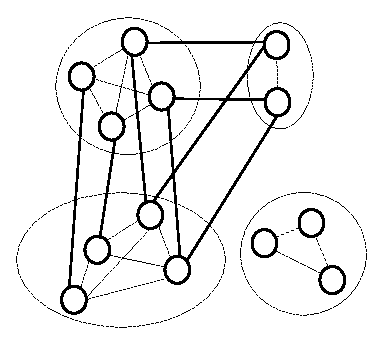
\includegraphics{figures/chapter3/fig_VRCillustrate.eps}  
\caption{References graph (solid-lines: relation edge , dashed-line: block edge)}
\label{fig:VRCillustrate}
\end{figure}

In step 3, the clustering is initialized by simply putting each reference node in single node cluster such that every reference has its own cluster. This is different from the original relational clustering algorithm where relational bootstrapping is necessary. In the initialization step, two lists are initialized in each node. The first list, we call the neighborhood list, contains information of the relational neighbor clusters. The second list,we call block list, contains information of the clusters that are in the same block that the node is.   

In step 4, the hierarchical agglomerative clustering start in each block. In each block, the two clusters having the highest similarity between them are searched. The search is restricted within each block. If the highest similarity is above the user-specified threshold, the two clusters are merged. upon merging the two clusters, all the relational neighbors (connected by relational edges) are notified. We use the block edges to store the values of the similarity between the corresponding clusters. When the cluster (represented by  vertex) need to find its highest similarity value it need to iterate through the list of its outgoing edges and choose the highest value. This is another difference to the original collective clustering algorithm that uses a priority queue to order the clusters merge.
When implementing the hierarchical agglomerative clustering in Pregel model, we need to follow the following steps:
\begin{itemize}
\item Finding the two clusters that have the highest similarity measure requires that each node communicates to all the other nodes within the same block. The method follows the following supersteps:
\begin{itemize}
\item In the first superstep, each node sends its attribute information as well as the information of its relational neighbor clusters to all other nodes in the block (by querying the block list). These information is used by the target node to compute the attribute and the relational similarity such that each node compute the similarity between it self and every other node in the block.
\item In the second superstep, each node compute its similarity against all the other nodes and propagate the highest similarity measure value computed by itself. When the other nodes receives this similarity measure value, they compare it to the values of similarity measure computed by them selves. If the receiving node finds that highest similarity value that is received from all the nodes, if this value exists within its computation then the node recognize that it has the highest similarity between it self and another cluster within the block, and they need to merge in this iteration. otherwise the node does nothing in this iteration and waits for the next iteration to check if the next highest similarity is within its computation.
\item In the third superstep, the two clusters with the highest similarity between them merges into new cluster. This requires unifying the cluster label, In addition, some extra work need to be done: 
\begin{itemize}
\item The neighborhood list of the new cluster need to be constructed by concatenating the neighborhood lists of the two merged clusters.

\item The block list of the new cluster need to be constructed by copying the block list from one of the merged clusters

\item The other clusters in the block need to update their block list by removing the entries of the old merged clusters and adding the entry of the new cluster

\item The relational neighbor clusters need to update their neighbor lists by removing the entries of the old merged clusters and adding the entry of the new cluster

\item Since the merge of clusters changes the relational structure of the reference graph, this effects the relational similarity, therefore the computation within all the blocks that include one of the relational neighbor clusters of the new cluster need to be done again. In fact this step gives the collective feature for the entity matching process. 
\end{itemize} 
\end{itemize}
\end{itemize}

Data partitioning is very important issue for the efficiency of our algorithm. We should aim for reducing the network overhead by having the blocks, each located completely in the same machine. Ideally, By assuring that data block are not distributed in many machines, we can have processing locally centered in each machine with minimum network traffic that is needed only when merging clusters since their neighbor clusters that need to be notified reside in other machines.

\subsection{Extending the Theoretical Foundation}

Now we are in good position to extend the theoretical foundation of the collective entity matching in order to be able to describe our vertex-oriented implementation of the collective entity matching approach. We start by having each reference in single element cluster, we use $C$ to denote the set of clusters $\mathcal{C}={c_i}$. We map each single-element cluster $c_i$ to a vertex $v_i$ in the graph $\mathcal{G}$ such that we have one-to-one mapping between single-element clusters and the vertices in the graph. Instead of the hyper-edges, we use bidirectional edges $E={e_i}$. Each edge can holds one value. This value is used to hold different values depending whether the edge is used to represent the relations between vertices (i.e. the references) or it is used to connect the vertices in the same block (i.e. similar references). 

Each vertex needs to send messages to the right vertices only. In order for the vertex to be able to do that, it needs to store and maintains four different lists. Considering that each vertex represents a cluster of references, we introduce the following notations for each cluster $c$:
\begin{itemize}
\item $c.B$: To denote the list of blocks that $c$ belongs to, we need this list since we use canopy blocking (i.e. overlapped blocks).
\item $c.BC$: To denote the list of block clusters, i.e. the clusters in the same blocks that $c$ belongs to. The vertex needs to send messages to clusters in this list when comparing references for matching.
\item $c.NC$: To denote the list of relational neighbor clusters, i.e the clusters that are connected to $c$ by relational edges. The vertex need to send messages to the clusters in this list only when it merges with another cluster. 
\item $c.MC$: To denote the list of merged clusters, i.e. clusters that are already merged with $c$. The clusters in this list need not to receive messages from $c$. 
\end{itemize}

The original collective relational clustering algorithm uses a priority queue to coordinate the priority of clusters merging in the agglomerative hierarchical clustering. In our vertex-oriented collective relational clustering, we use the value attribute of edges that connect vertices in the same block to store the similarity value between the cluster and the other clusters that the edges towards to instead of using a single priority queue. The vertex (i.e. cluster) needs to iterate through its outgoing edges in order to get its similarity with all other clusters in the block. This solution have many desired benefits:
\begin{itemize}
\item It gives another usage of the block edges in addition to sending messages
\item It avoids the problem of priority queue exhausting that is one of restrictions of the original collective relational clustering algorithm
\item It is more natural to the graph structure 
\end{itemize}
    
\subsection{Mathematical Foundation of the Communication}
We can model our algorithm as a \textit{Channel systems}\cite{BaKa08}. Channel systems are popular for describing communication protocols. We give the intuitive definition of the Channel systems from \cite{BaKa08}: 


Intuitively, a channel system consists of $n$ (data-dependent) processes $P_1$ through $P_n$.
Each $P_i$ is specified by a program graph $PG_i$ which is extended with \textit{communication
actions}. Transitions of these program graphs are either the usual conditional transitions, or one of the communication actions with their respective intuitive meaning:
\begin{quote}
$c!v$ transmit the value v along channel c,
\newline
$c?x$ receive a message via channel c and assign it to variable x.
\end{quote}
Channels are first-in, first-out buffers that may contain messages. Considering channel c as buffer, the communication action $c!v$ puts value $v$ (at the rear of) the buffer whereas $c?x$ retrieves an element from (the front of) the buffer while assigning it to $x$. Let

\begin{quote}
$Comm$ = $\lbrace$ $c!v$, $c?x$ $|$ $c \in Chan$, $v \in dom(c)$, $x \in Var$ with $dom(x) \supseteq dom(c)\rbrace$
\end{quote}

denote the set of communication actions where $Chan$ is a finite set of channels with typical element $c$.

A channel $c$ has a (finite or infinite) \textit{capacity} indicating the maximum number of messages it can store, and a type (or \textit{domain}) specifying the type of messages that can be transmitted over $c$. Each channel $c$ has a capacity $cap(c) \in \mathbb{N} \cup \lbrace \infty \rbrace$, and a domain $dom(c)$. For a channel $c$ that can only transfer bits, $dom(c) = {0,1}$. If complete texts (of maximum length of 200, say) need to be transmitted over channel $c$, then another type of channel has to be used such that $dom(c) = \sum^{\leq200}$, where Σ is the alphabet that forms the basis of the texts, e.g., $\sum$ is the set of all letters and special characters used in German texts.

The capacity of a channel defines the size of the corresponding buffer, i.e., the number of
messages not yet read that can be stored in the buffer. When $cap(c) \in \mathbb{N}$, $c$ is a channel with finite capacity; $cap(c) = \infty$ indicates that c has an infinite capacity. Note that the special case $cap(c) = 0$ is permitted. In this case, channel $c$ has no buffer. Communication via such a channel $c$ corresponds to handshaking (simultaneous transmission and receipt, i.e., synchronous message passing) plus the exchange of some data. When $cap(c) > 0$,
there is a "delay" between the transmission and the receipt of a message, i.e., sending and
reading of the same message take place at different moments. This is called asynchronous
message passing. Sending and reading a message from a channel with a nonzero capacity
can never appear simultaneously. By means of channel systems, both synchronous and
asynchronous message passing can thus be modeled.

We can map our algorithm to the Channel systems model such that the vertex corresponds to the process in the Channel systems model, Supersteps corresponds to the states of the program graph and the edge corresponds to the channel.

\subsection{Complexity Analysis}
We have two sets of graphs. The first set is the set of graphs built by adding the  
\subsection{Multi-type Entity Matching}
Out framework supports multi-type entity matching. Different types of entities are connected by the relational edges in the relational graph. Then the references belong to each entity type is blocked such that similar references that belong to the same entity type are compared for matching. In the implementation we tag the type of entity.
When building the relational graph we connect instances of different entity types by relational edges to form a complete graph, i. e. every two vertices are connected by an edge.

Lets see how this is applied for our running example. Lets say that it is required to match the paper references  in addition to matching the author references. Here we have multi-type entity matching where author references are matched and papers references are matched in the same task. All the references of different types are connected by the relational edges such that each two vertices are connected, this lead to having a complete graph. Figure \ref{fig:multitypeEdges} shows papers $P1$ and $P4$. References to different types of entities (author and paper entity types) are connected by relational edges such that for each paper we have a complete graph (every twp vertices are connected). Then similar references that belong to the same entity type are blocked and block edges are used to connect the vertices corresponds to these references.

\begin{figure} 
\centering
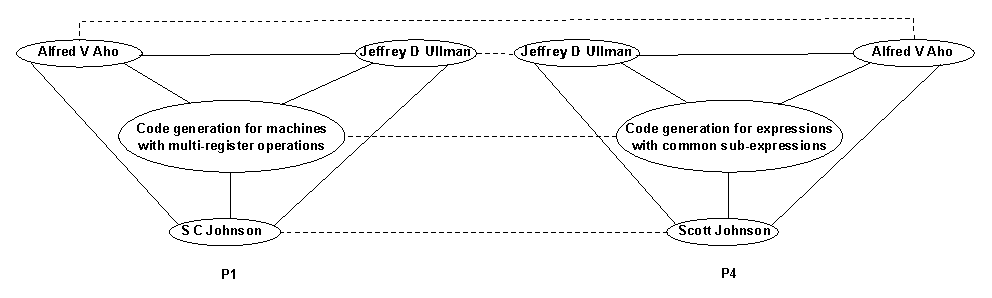
\includegraphics{figures/chapter3/fig_multityperelations_example.eps}  
\caption{multi-type references (solid-lines: relation edge , dashed-line: block edge)}
\label{fig:multitypeEdges}
\end{figure}
 

\subsection{Canonicalization}
Canonicalization is the construction of cluster representative with maximal information by combining information from its cluster elements.
We implement this in our entity Info data structure.

\subsection{Optimizing for the Cloud}
Graph applications composed using the Pregel/BSP model encounter performance and scalability bottlenecks for applications that exhibit a log-normal distribution in messages exchanged during the supersteps when operating on small world graphs. this sharply ramp up the cumulative messages exchanged between supersteps as their traversals reach supernodes in the small world graph, and drain down with a long tail of supersteps whose total number typically corresponds to the graph’s
diameter. Issues with scalability for applications with variable message exchange patterns arise due to the corresponding changes in resources required over different supersteps that can lead to costly (money) over-provisioning or costly (time) underprovisioning of partition workers. On BSP frameworks messages must be buffered since they must be delivered by the end of a superstep but not drained (processed) until the next. This can be done either using (costly) disk access or by
retaining them in memory, leading to memory pressure. We would like to maximize memory utilization for buffering messages without spilling over to virtual memory on disk, which
may be even worse than disk-based buffering due to virtual memories random access (vs. sequential for disk-based buffering) I/O patterns.

Redekopp et al. proposed a vertex-scheduling model for Pregel/BSP, where computation for only a subset, or swath, of vertices is initiated at a time, though that computation may require action from all vertices in the graph as a traversal progresses. This approach allows resource utilization to be spread over time and shaped based on the swath size and the initiation interval between swaths. Clearly the swath size should be set as large as possible to provide good
utilization but small enough to allow messages during peak supersteps to fully reside in physical memory.
\section{Adaptive/Incremental Entity Matching}
\section{Graph-based Data Warehouse} 